\documentclass[../main.tex]{subfiles}

\begin{document}
\section{Theory}\label{sec:theory}
  \subsection{Franke's function}
Franke's function is a function which is quiet often used to test different regression and interpolation methods. The function has two Gaussian peaks of different heights, and a smaller dip, which makes it quiet convenient for testing interpolation methods and algorithms. The function reads as follows:

\begin{align*}
f(x,y) &= \frac{3}{4}\exp{\left(-\frac{(9x-2)^2}{4} - \frac{(9y-2)^2}{4}\right)}+\frac{3}{4}\exp{\left(-\frac{(9x+1)^2}{49}- \frac{(9y+1)}{10}\right)} \\
&+\frac{1}{2}\exp{\left(-\frac{(9x-7)^2}{4} - \frac{(9y-3)^2}{4}\right)} -\frac{1}{5}\exp{\left(-(9x-4)^2 - (9y-7)^2\right) }.
\end{align*}

The functions defined interval is $x,y\in[0,1]$. The shape of the function can be seen in figure \ref{fig:frankesplot}

\begin{figure}
\centering
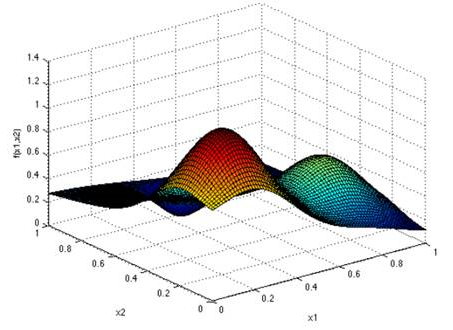
\includegraphics[width = 3in]{frankesfunction_plot.png}
\caption{Shape of Franke's function which will be used as a interpolating goal.
\\Note to self: Might be better to plot the graph instead of using a figure from the web. Remember to add the source for the figure by using for example bib. https://www.sfu.ca/~ssurjano/franke2d.html}
\label{fig:frankesplot}
\end{figure}

\end{document}
